\chapter[Our Fond Memories Of GR]{Our Fond Memories Of GR}\label{chap20}

\Authorline{GR's Family Members}

\authinfo{%
Memorable pictures in our mind\\
Live in the album of hearts forever!\\
GR Family%
}

\begin{figure}[H]
\centering{
\includegraphics[scale=.3]{figures/chap23-fig1.eps}
}
\end{figure}

\section*{My Good Memories Together}

In our Journey of 63 years together, I have experienced and learnt many good things in my life. Our relationship was a strong bond and we embraced life as it came and never had any big materialistic aspirations. We used to accept challenges and happiness as part of life, So, It has been a wonderful life journey. As parents, we enjoyed kids growing up and selecting their studies and careers. He always stood like a rock supporting them to give his best when it came to their education. This is because he firmly believed in two things: 1.Surrendering to God and Guru while focusing on daily activities. Even today I feel that he is among us, as we practice the simple lifestyle taught by him. In his last days his very presence was touching our hearts like a Spiritual Guru. 

My sincere prayers to God to keep him Happy for ever…
\bigskip

\hfill\textbf{Mrs. Seethalakshmi Ramachandran}

\newpage

\section*{ My dear Brother – GR}

\noindent \textbf{My dear Anna,}

\textbf{I recall in the late Forties}, when I was a small boy, you taught me the basic tenets of Bhakthi, by performing Alankara to the copper idol of Sri Venkateswara daily, during Utsava days, decorating in different ways each day.

\textbf{I recall in the early fifties}, in your college days when I spent a year away from Chittoor , with our family @ Tambaram, you made sure that I didn’t miss my school by giving me home work when you left for college and made sure that I completed it by the time you returned home.

\textbf{I recall in the mid fifties}, when you were alone @ Chennai and I and parents were at Chittoor , how I eagerly awaited your home coming during your holidays, just to hear from you about the interesting anecdotes from life @Madras Christian  College (MCC) including about classic novels that you read from the library.

\textbf{I recall} your grand wedding and my upanayanam, both of which were celebrated @ Trichy and the home coming of my sister in law to Chittoor.

\textbf{I recall in the early sixties}, at Chennai when I just entered MCC for PU and with father having retired, how as a young Research Scholar, you shouldered the responsibility of the entire family and encouraged me to continue my studies although I offered to take up a job after PU.

\textbf{I recall} in 1964, how both of us received our respective degrees at the same convocation of the Madras University PhD for you and BSc for me, both in Physics.

\textbf{I recall} in 1964, how you managed to apply on my behalf for admission to Electronics Engineering @ Madras Institute of Technology (MIT), when I was really away with our beloved father @Sri Kalahasthi in AP.

\textbf{I recall} in 1965, you left MATSCIENCE in disappointment for ISI- Calcutta as a Post Doc and later shifted the family there, with me joining the Hostel @ MIT.

\textbf{I recall} in 1967, when our beloved father suddenly left for his heavenly abode, you received me in a state of daze @ Howrah Rly Stn, my having travelled from Bombay, where I was taking my training @ TIFR post my Engg @ MIT.

\textbf{I recall how from that moment on, how you guided me all through my life more like a parent than a sibling, getting me married to a lovely \& devoted partner so that my life bloomed, till that momentous 9th day in April 2020, when you breathed your last.}

\textbf{This is my tearful farewell My Dear Anna, I am sure that God in whom you reposed your faith all through the different phases of your life , some trying, some turbulent and many in later years more pleasant and happy with your beloved Children and Grand Children and your Dearest Students, who earned as much of your love \& affection as myself, will ensure that you attain Eternal Peace at His Lotus Feet. } 

\bigskip

\begin{flushright}
\begin{tabular}{c}
\multicolumn{1}{p{3cm}}{\textbf{Aum Shanthi}}
\end{tabular}
\end{flushright}

\noindent \textbf{With as much Love and Affection as I received from you}
\bigskip

\hfill Your Dear Viswam

\hfill \textbf{G. Viswanathan}

\newpage

\section*{GR as dad, Guru and Beyond…}

We as kids grew up in a traditional Orthodox family which emphasized more importance for values in life. My dad was not a kind of person who would go out on socializing with people across the society or picnics to enjoy life. He had his style of doing things by being grounded to core values of life. Having said that, he had given full freedom in choosing everything right from studies, employment, life partner etc. I can say he had given the biggest gift to me - which is - he firmly believed in me. When I decided to move to Bangalore for my career progression, he had only one advise - Focus on your job, give your best, believe in god / Guru \& the rest will follow you. This advice made me a balanced individual today \& grounded with core values in life and not forgetting my roots. He has molded me in the right path \& has done a beautiful handholding without physically present with me. Memories to cherish forever.

\bigskip

\begin{flushright}
\begin{tabular}{c}
\multicolumn{1}{p{2cm}}{\textbf{Ramakrishna}}
\end{tabular}
\end{flushright}

\newpage

\section*{About Father}

It is very difficult to describe Father with few adjectives, but here is how I remember him and admire these qualities – Dedicated, Principled, Brilliant and Simple.

His faith \& dedication to God was something that he demonstrated under all circumstances. His dedication to our family, his work and students always came before his needs.

Such was his passion \& love for his work that he actively pursued it for 20+ years after his retirement. He was always surrounded by students \& was very generous with his time and resources towards them. Doors were always open and never seen him refusing anyone who sought his guidance.

He was very principled and had few fundamental beliefs and rules which he followed with steadfast resolve irrespective of the situation, be his daily routine, food habits, his devotion to God. This grit and determination have instilled a sense of awe in us and it is difficult for us to emulate. Life lessons we learnt from him are family values, honesty, integrity empathy and rightfulness. Irony is, he neither used these words not talked about them. It was for us to see through his actions.  

His brilliance requires no introduction! Beside brilliance he had this uncanny ability to distill the essence of any subject/ concept and present it. He was gifted with psychic like ability to read through your mind to see if you are able to follow him. His ability to explain complex concepts in simple language captivated his audience the most. It is very difficult to find a teacher with these exceptional qualities. 

A person with his magnitude of work and achievements could have lived an exuberant life however chose the path of simplicity. He always led a life with what is necessary and materialistic things were never important for him. We have always seen him help people in need to the extent possible. 

As I got older, I came to appreciate that his guiding principles has had influence on every aspect of my life.  And when I’m at my best, I know it is because of what he taught me that made it possible. 

As I conclude, realize the best way to express my gratitude to him is to embody the values he gifted us. 

‘Greatest Dad’ may sound cliché, but I can’t Thank you enough Nayana. You are always with us and within us.
\bigskip

\begin{flushright}
\begin{tabular}{c}
\multicolumn{1}{p{2cm}}{\textbf{Krishnakumar}}
\end{tabular}
\end{flushright}
\newpage

\section*{My Treasured Memories of Father}

There is a special kind of feeling when I think about Father.  Not a single day goes by that I don’t think about my dear father.
\medskip

Focusing on all the incredible memories, so vivid and special are my memories of early childhood days spent in Calcutta with my father. To me, father was a smart, brilliant, simple and honorable figure. I still remember those evening walks I took with my father. Holding his hand, I would walk long distances in the streets and lanes of Calcutta shopping little things, eating my favorite Ice creams that my father used to buy almost every day for me. Another occasion that made me very excited was the long train journeys with my father, mother and brother.
\medskip

Father remained a pillar of strength, support and discipline to all of us. He always had something valuable to share with us all that we always respected. We all enjoyed nice story time when father used to narrate inspiring stories from Ramayana, Mahabharata and Bhagavatham to imbibe good values along with our regular studies. I feel I’m very lucky to have had such a wonderful father whom I consider as a special person in my life. When it came to the choices of our courses and subjects, father would always say that it is important for us to make our choices and be happy with our decisions.
\medskip

We all siblings have an emotional attachment to the house R-10 (University Quarters) where we all grew up with fond memories. It is our precious memories of the days spent with our Father, Mother, Grandmother that really made that house into a lovely home. The garden of that house we all loved had many memorable trees and fragrant flowers. Each room in that house fills our memories with people we lived, the tender moments and the fun we all enjoyed together that can never be forgotten.
\medskip

I firmly believe that Father’s guidance has shaped me the person I’m today. I’m also grateful for my loving Grandmother who has brought us up by showering her love and shaped our personality. My mother always bound by her duties is an example of selfless love and sacrifice for our family. Another person whom I wanted to share my regards is my loving uncle who has always been our support and enthusiasm and shared much of our family responsibilities which I can never forget. 
\medskip

Though Father is physically away from us, he is ever fresh in our hearts and memories.
\medskip

I’m sure Father’s incredible legacy of knowledge lives on forever and continues to be loved and appreciated by many… 
\medskip

My sincere prayers to My dear Father… 
\bigskip

\begin{flushright}
\begin{tabular}{c}
\multicolumn{1}{p{2cm}}{\textbf{Latha}}
\end{tabular}
\end{flushright}
\newpage

\section*{My precious memories of Father}

As far as I can remember I have had a happy childhood. My parents handled my wrongdoings and mistakes very calmly, although I can’t remember doing something that’s very bad. Being a girl in my family, I think helped on making my punishments not that painful. But how my parents raised me is what made me the person that I am today, and I think they did a great job.
\medskip

When I look back to my childhood days, I recall many things that give me joy even today. My childhood memories are those of a sheltered and carefree life, cherished with love and affection. My dad was a kind, loving and a self-disciplined man I know. I still remember those sunny afternoons he would pick us from school and take us to visit the Zoo, Chamundi hills or Cauvery art. I cherish and treasure those simple things that we did together with dad. I can still taste the chocolates he would buy us on his way home from work every day. Those early memories include having Dad help me with learning math and English and visiting his office at the university, where I was fascinated by the room with a large black board and a box full of colored chalk. I have to thank my father for my problem-solving skills, and for a determination to get things done and never give up until satisfied.
\medskip

I am lucky in many ways. I was taught by my dad to be fair, independent and to believe in God. If someone has a hard time, do not put the person down. Make sure that the weakest have their share. Have faith in God. Situations can sometimes lead to isolation or confusion. When you feel hopeless or lost you can find rest and comfort in the love of god. Dad gave us numerous instances from Ramayana and Bhagavata to show how God comforts and gives you wisdom in times of darkness and confusion. Not only me, but everybody around my father, has been learning these facts of life.
\medskip

Different personality traits make us who we are today. There are many factors to our personalities and each aspect illustrates a bigger picture of who we are and how we came to be. My parents shaped me into the person I am today. I have been raised in a very close-knit family, and every night without exception my whole family gathers together to enjoy a good home cooked meal, and the time spent with each other. We grew up celebrating all festivals together at home with our dad being the center of it all. Deepavali was always my favorite. My fondest memories are of every Deepavali morning as a child, my five siblings and I would all wake up at 4:00 am, and light up fire crackers with our dad. At home, we have a tradition where we wake up early morning, light up fire crackers and our grandmother would fondly smear warm gingelly oil on the head and face followed by the traditional oil bath. My most memorable Deepavali was when my uncle and aunt also joined us during those celebrations. The fire crackers, new dresses and the homemade sweets was truly magical! 
\medskip

I have been raised by what most people would consider to be old school orthodox parents. I am so grateful for this upbringing, and I'm so appreciative of the two people who made me into the woman I am today. My family has impacted my life substantially when it comes to my physical, social, and emotional development. I have established most of my own morals, beliefs, and values based upon the way I was raised by my parents.
\medskip

There’s no denying the power and influence dads have on their daughters’ upbringing and transformation into young women. My sisters and I were raised in a household with a very authoritative, strong dad to whom I attribute many of the lifelong lessons I’ve learned. He always taught us to be as respectful as possible, at all times, to all people. My dad was there to coach and mentor us during our most crucial teen and adult years. I believe that the support received from dads is very important in the upbringing of strong, independent women. My dad and I may not share the same gender, but many of the unexpected little things I've learned specifically from him have impacted my continuous growth into a woman.
\medskip

My father has always been a supportive voice of reason for all of my educational and career decisions and it remained so until his last day. I always felt blessed that my dad, found a way to prioritize my education above everything else. He gave me the precious gift that all great parents and teachers give: the power to think for myself. The point is that it's more worthwhile to teach people to do something for themselves than it is to do it for them. Looking back, I realize he wasn't just teaching me how to solve a math or a physics problem, he was laying a safe path for my life journey.
\medskip

In my eyes as a child, no one was more powerful than my dad, who I consider to be "The Strong Man." He couldn't lift mountains with one hand, but his personality and presence were striking enough that when he needed to intimidate or make an impression, he sure did. I will never know what it's like to be in the shadows of a meeker dad, and thankfully, since my dad raised me to be as strong as him, I have my own spotlight and will never lurk in the crowd. 
\medskip

I am very proud to be his daughter and I can proudly say that my father has been my source of inspiration. In other words, his perspective and personality together have shaped me as a person. He will be dearly missed, as his impact continues onward.
\bigskip

\begin{flushright}
\begin{tabular}{c}
\multicolumn{1}{p{2cm}}{\textbf{Devi}}
\end{tabular}
\end{flushright}
\newpage

\section*{Father}

- A unique feeling… Father
\medskip

To the rest of the world, he is Professor G Ramachandran, DR. G. Ramachandran, Scientist  G. Ramachandran, etc.but for me, he is my beloved father, G. Ramachandran. 
\medskip

When I once roll back to my childhood, I am able to view the happy, smiling and angry faces of my father. A very confident, simple, contended person., and a great believer of God. No doubt, he was a strict father. but the knowledge that I gained from my father has helped me today to understand the world. My father was very affectionate and supportive. He encouraged me to pursue my studies in my field of interest. He used to recite Bhagavad Gita, Ramayana and Mahabharath and explain the meaning of each and every sentence clearly. 
\medskip

I am not able to believe that, my father is not with us anymore. I am sure that he is happy somewhere and watching us.

\bigskip
\begin{flushright}
\begin{tabular}{c}
\multicolumn{1}{p{2cm}}{\textbf{Gowri}}
\end{tabular}
\end{flushright}

%\newpage

\section*{My Dad through My Eyes}

Dad, you are a man like no other. You taught me discipline, humanity and ethics of life. You continue to be a powerful influence in all my achievements.

I’m still your little girl waiting for your chocolates, but today, I feel insecure without your unconditional care and concern. You taught me everything except how to live without you.
\bigskip

\noindent I MISS YOU NAYANA.

\noindent Love you

\begin{flushright}
\begin{tabular}{c}
\multicolumn{1}{m{2cm}}{{\centering \textbf{Buvvai} \\ ~~~\textbf{Anuradha}}}
\end{tabular}
\end{flushright}

\newpage
